\documentclass[11pt,BCOR2mm,DIV14]{scrartcl}
\usepackage[Glenn]{fncychap}
%For symbols in T1 encoding.
\usepackage{textcomp}
\usepackage[colorinlistoftodos, textwidth=4cm, shadow, textsize=tiny]{todonotes}
\usepackage{amsmath,amsfonts,graphicx,ncsg3,comment,typearea,pifont}
\usepackage{xcomment,color, psfrag,enumerate,scrpage2,xspace,listings,wasysym, 
comment}
\usepackage{termcal}

%For fancy tables
\usepackage{booktabs}

%For symbols in T1 encoding.
\usepackage{textcomp}
\begin{document}

\section*{Thoughts}

To get things rolling, I thought we could use the model below - if we can't make progress with this model, then more complicated processes aren't really an option! This is only a thought, I'm happy for other suggestions.

At the end, I've given a couple of associated inference problems. In particular, the likelihoods in figure \ref{F2} are \textit{banana shaped}, and so exploring the space could be tricky. 

\section*{Immigration death model with counts}

This model has two species, $N(t)$ and $C(t)$. The first reaction represents a constant immigration rate, and occurs with rate $\alpha$. The second reaction represents death in the $N$ population and occurs with rate $\mu N(t)$. The model can be represented by the coupled (pseudo) reactions, 
\begin{equation}\label{1}
R_1: \emptyset  \xrightarrow{\phantom{a}\alpha\phantom{a}} N 
\quad \text{and} \quad
R_2: N  \xrightarrow{\phantom{a}\mu\phantom{a}} C .
\end{equation}
Essentially, species $C(t)$ is the number of deaths that has occurred up until time $t$. Hence, species $C$ is a monotonically increasing\footnote{This model is used in physics, where photons of light are fired into a box and we only observe photons leaving the box.}. The forward Kolmogorov equation (or CME) for this model is
\[
dp_{nc}(t)/dt = \alpha p_{n-1, c}(t) +  \mu (n+1) p_{n+1,c-1}(t) 
- (\alpha + \mu n) p_{nc}(t) \;.
\]
This equation can be solved exactly using a generating function approach.

\subsection*{Moments}

The general idea of \textit{moment closure} is to represent the analytically intractable moments of the process as a set of ODEs. The solutions of these ODEs provide approximations for the moments. With this particular system, we can solve the ODEs analytically - so the moments are exact.

The marginal means of the process are:
\begin{align*}
E[n(t) | n(0) = n_0 ] &= \frac{\alpha}{\mu}(1-e^{-\mu t}) + n_0 e^{-\mu t} \\
E[c(t) | n(0) = n_0, c_0=0] &= \frac{\alpha}{\mu} (\mu t + e^{-\mu t} - 1) + \alpha n_0(1-e^{-\mu t}) \;.
\end{align*}
Notice that as $t \rightarrow \infty$,
\begin{align*}
E[n(t) | n(0) = n_0 ] &= \frac{\alpha}{\mu}\\
E[c(t) | n(0) = n_0, c_0=0] &\simeq \alpha t + n_0 \;.
\end{align*}
The marginal variances are a bit more messy, but still fairly tractable:
\begin{align*}
Var[n(t) | n_0]  &= \left(\frac{\alpha}{\mu} + n_0e^{-\mu t}\right)(1-e^{-\mu t})\\
Var[c(t) | n_0, c_0=0]  &= \frac{\alpha}{\mu}(e^{-\mu t} - 1) + \alpha t + n_0 \mu e^{-\mu t} - \frac{n_0 e^{-2\mu t}}{\mu} \;. 
\end{align*}
The covariance for $N$ and $C$ is
\begin{align*}
E[n(t), c(t)| n_0, c_0=0] &= \frac{\alpha^2}{\mu^2}(-1+e^{-\mu t}+\mu t)(1-e^{-\mu t}) + 
\frac{\alpha}{\mu} (-1+e^{-\mu t}+\mu t) n_0 e^{-\mu t} + \\
&\quad +\frac{\alpha}{\mu} (1-e^{-\mu t})^2 n_0 + 
n_0^2  (1-e^{-\mu t})e^{-\mu t}
- n_0(1-e^{-\mu t})e^{-\mu t}\;.
\end{align*}


\section*{Inference}

Two possible scenarios that I've looked at in the past are:
\begin{enumerate}
\item We observe species $N$ at discrete time points $t_0, t_1, \ldots, t_{n+1}$. Assuming no error in the observations and a uniform prior, we obtain the likelihood (or posterior) surfaces shown in figure \ref{F1}.
\item We observe all deaths in the process, i.e. we observe species $C$ exactly. Here we get likelihood/posterior surfaces of the type in \ref{F2}
\end{enumerate}
In both cases, there is no observation error involved. Ironically, this actually makes inference very tricky in an ABC/MCMC. Since we need our simulations to exactly hit the target.

\begin{figure}[h]
\centering
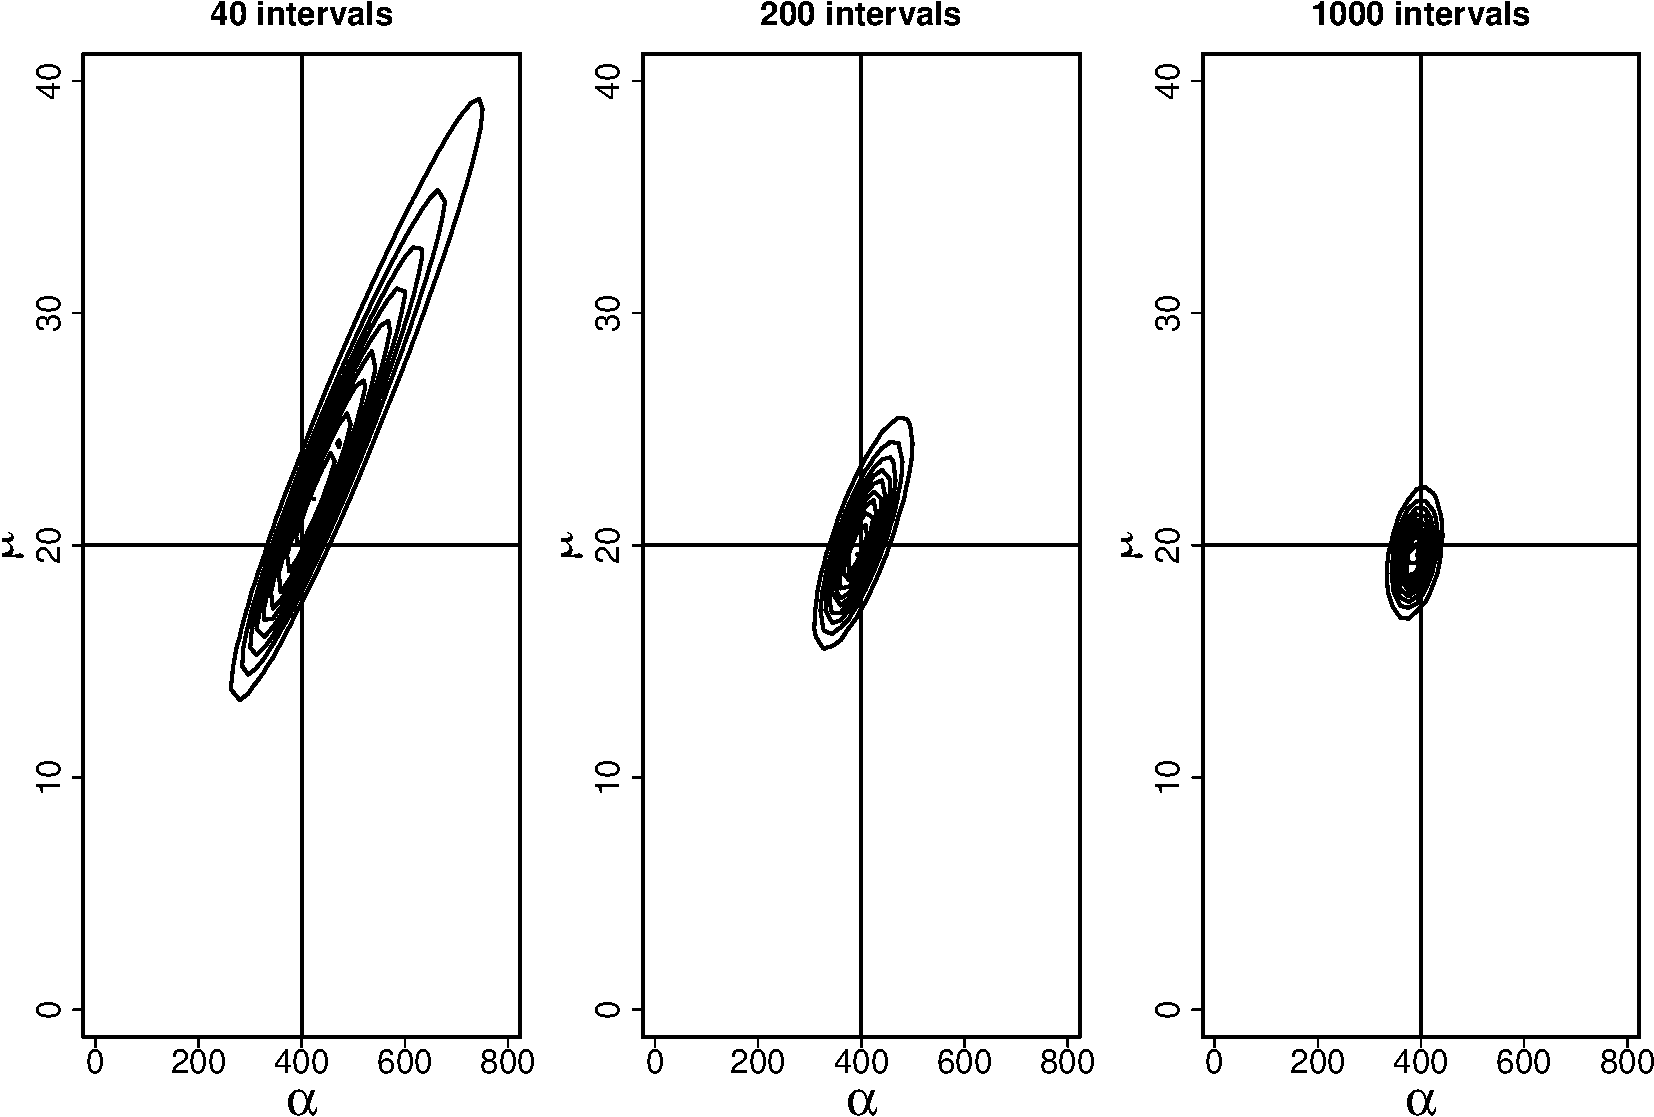
\includegraphics[width=0.8\textwidth]{graphs/likelihood_disc_2-crop}
\caption{Plots to show the exact discrete time point likelihood, for $\alpha =400$, $\mu=20$ and $n_0=0$.}\label{F1}
\end{figure}
\clearpage
\newpage
\begin{figure}[t]
\centering
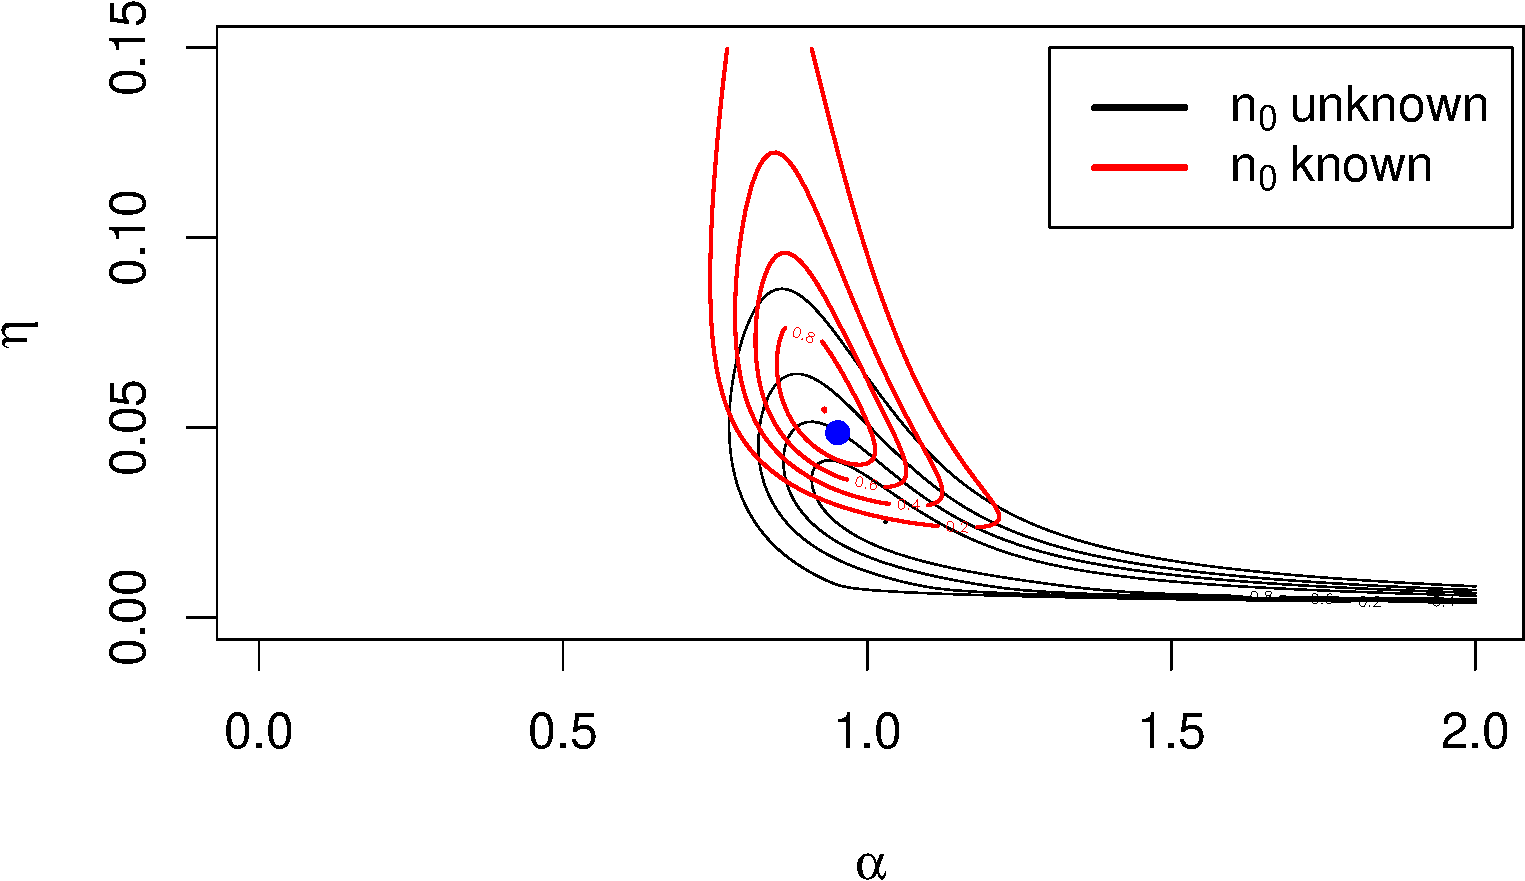
\includegraphics[width=0.8\textwidth]{graphs/n0_0-crop}
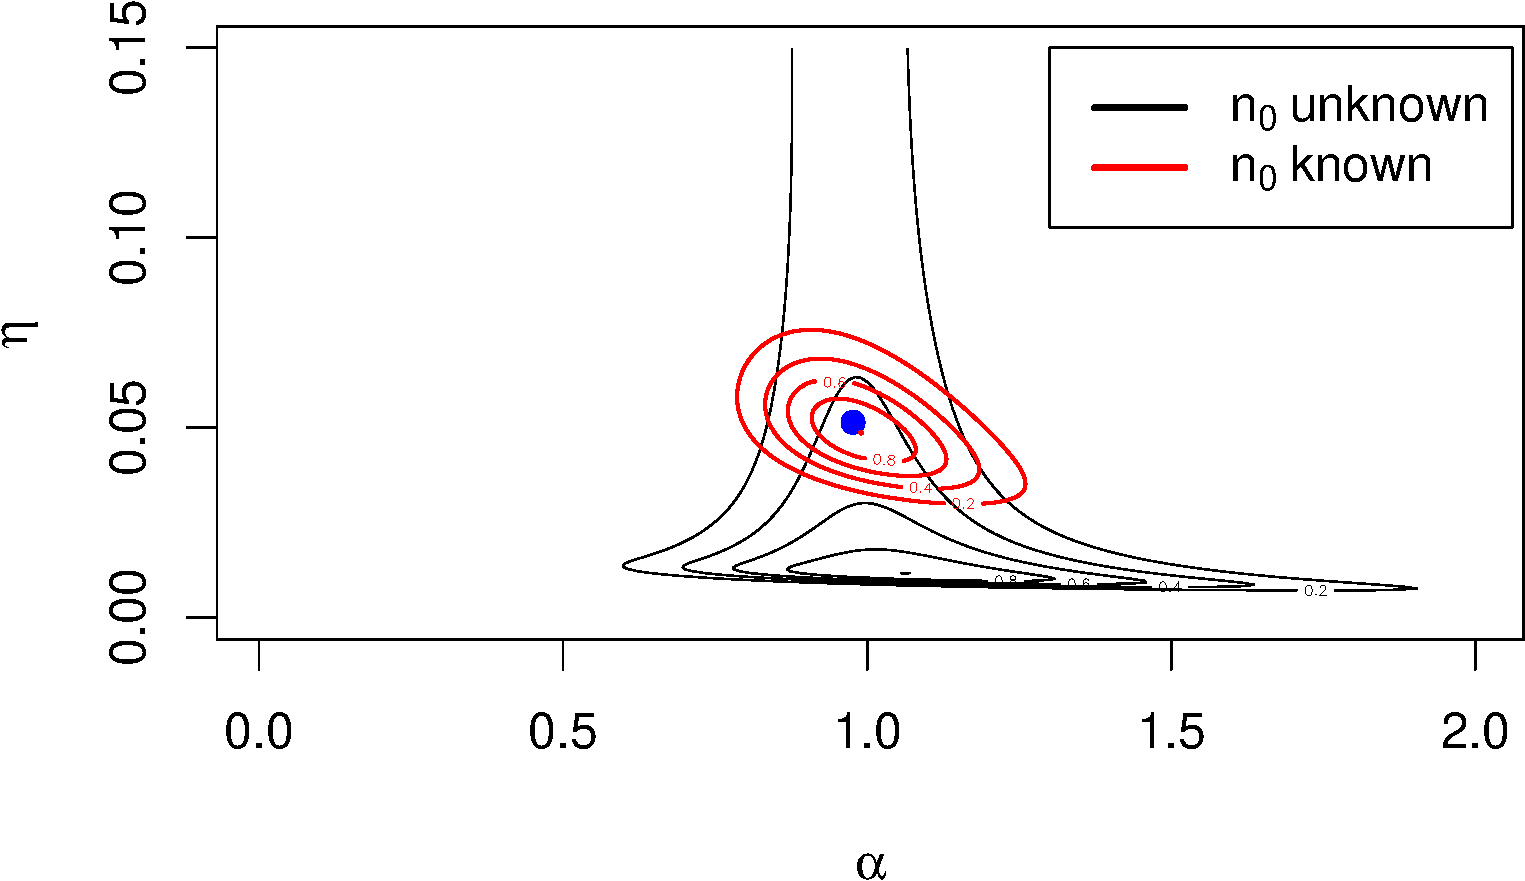
\includegraphics[width=0.8\textwidth]{graphs/n0_20-crop}
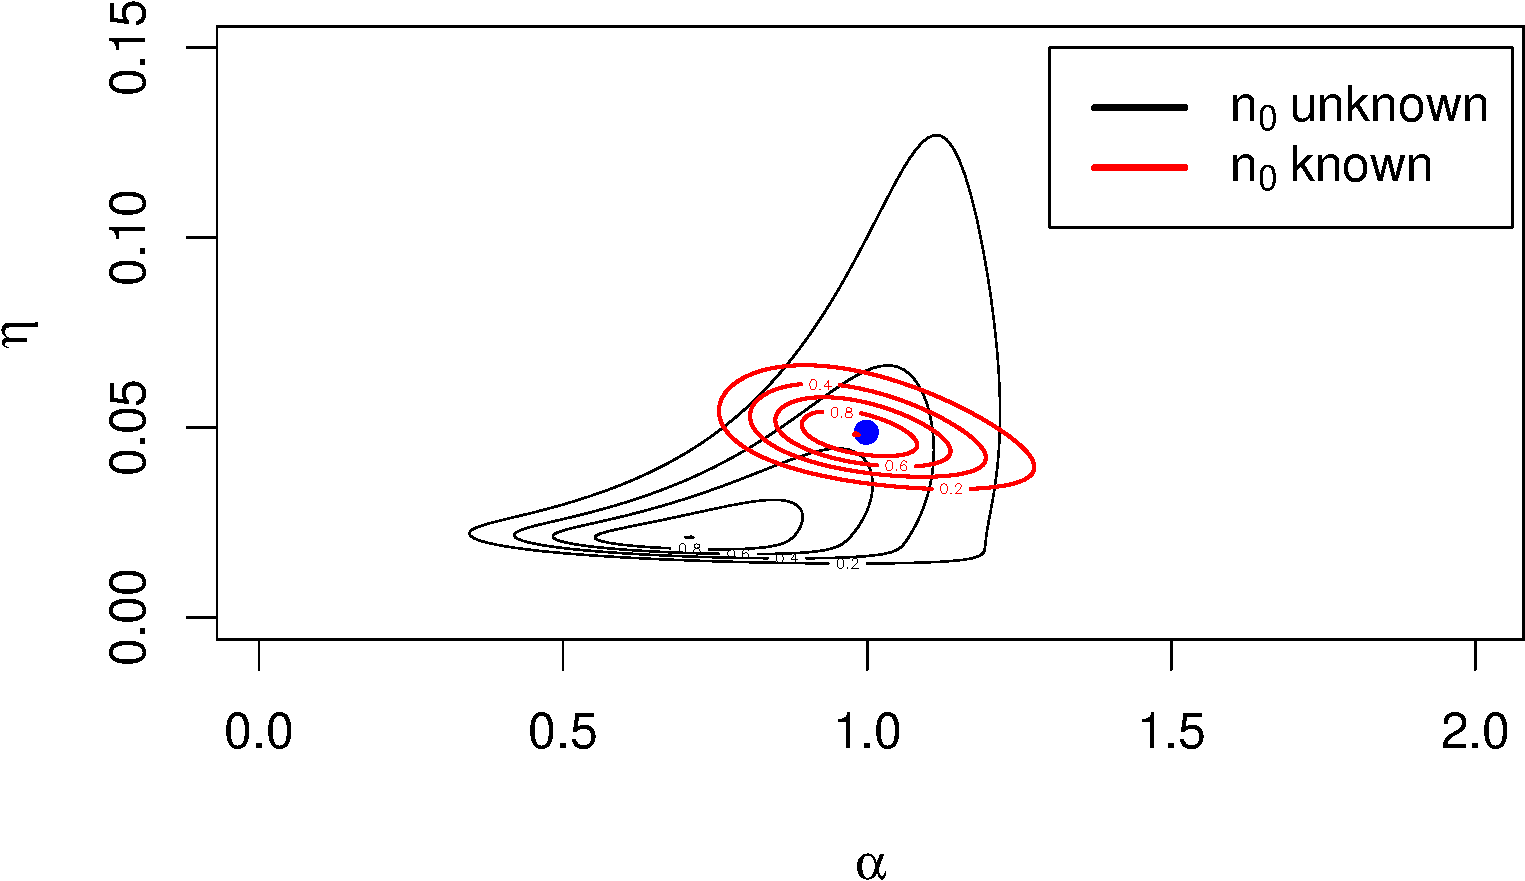
\includegraphics[width=0.8\textwidth]{graphs/n0_40-crop}
\caption{Likelihood surface plot using the 100 death times from a single realisation, when the initial population is known (red) and unknown (black). Parameters were $\alpha = 0.05$, $\mu=0.05$ and (a) $n_0=0$, (b) $n_0 = 20$, (c) $n_0 = 40$. The true parameters are shown as a blue dot.
Note: the $y$-axis label should be $\mu$ not $\eta$.}\label{F2}
\end{figure}


% 
% Following \citet{Matis06}, we assume a linear aphid population birth rate of $\lambda N(t)$ where 
% $N(t)$ denotes the size of the aphid population at time $t$. As discussed in \citet{Prajneshu98}, aphids 
% excrete honey-dew, forming a cover on the leaf surface and causing aphid starvation. As the area covered by excretion 
% at time $t$ is proportional to the cumulative population size at time $t$, $C(t)$, we assume a death rate 
% of $\mu N(t)C(t)$ and for simplicity, assume that there is no removal or decomposition of honey-dew 
% \citep{Matis06,Matis07a,Matis08}. The model can be represented by the coupled (pseudo) reactions, 
% \begin{align}
% N & \xrightarrow{\phantom{a}\lambda\phantom{a}} 2N + C \label{2.1} \\
% N+C & \xrightarrow{\phantom{a}\mu\phantom{a}} C \label{2.2}
% \end{align}
% since clearly, an occurrence of (\ref{2.1}) will lead to a unit increase in both $N$ and $C$ whereas the reaction in  (\ref{2.2}) will give a unit decrease in $N$ but leave $C$ unchanged. Such models are known in the literature as stochastic kinetic models; see \citet{Wilkinson06} for a concise introduction. We can express the probabilistic laws governing the time evolution of the process by considering a small interval $(t,t+dt]$, namely
% \begin{align}
% \Pr\left\{N(t+dt)=n(t)+1,\,C(t+dt)=c(t)+1\,|\,n(t),c(t)\right\}&=\lambda n(t)dt+o(dt) \label{2.3} \\
% \Pr\left\{N(t+dt)=n(t)-1,\,C(t+dt)=c(t)\,|\,n(t),c(t)\right\}&=\mu n(t)c(t)dt+o(dt),\label{2.4}
% \end{align}
% and we adopt the convention that upper case denotes random variable and lower case denotes the realisation. 
% The expressions in (\ref{2.3}) and (\ref{2.4}) describe a Markov jump process where each event occurs at a particular rate dependent on the current state of the system. Note that ignoring stochasticity leads to a deterministic model where the time course behaviour of 
% $N(t)$ and $C(t)$ is described by the set of differential equations,
% \[
% \left\{\begin{array}{l}
% \displaystyle\frac{dN(t)}{dt}=\lambda N(t)-\mu N(t)C(t)\\
% \\
% \displaystyle\frac{dC(t)}{dt}= \lambda N(t)
% \end{array}\right.
% \] 
% 
% 
% 
% 
% 
% 
% Suppose we have two species $X$ and $C$. 
% \[
% R_1: \emptyset \xrightarrow{\alpha} X 
% \quad \text{and} \quad 
% R_2: X + C \xrightarrow{\mu X C} 2C
% \]
% 


\end{document}